
\section{SSTV}
\label{section:sstv}
\begin{frame}%STARTCONTENT

\frametitle{Slow-Scan-Television (SSTV)}
\begin{itemize}
  \item Beim Slow-Scan-Television (SSTV) werden stehende Bilder mit geringer Auflösung übertragen.
  \item Rufzeichen und Rapporte werden bei SSTV einfach als Text in die Bilder reingeschrieben.
  \end{itemize}

\begin{figure}
    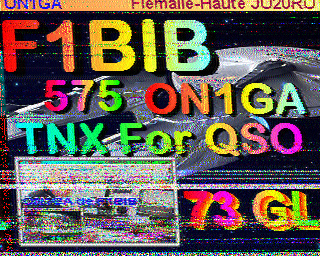
\includegraphics[width=0.85\textwidth]{foto/84}
    \caption{\scriptsize Ein per SSTV übertragenenes Bild}
    \label{n_sstv}
\end{figure}
\end{frame}

\begin{frame}
\only<1>{
\begin{QQuestion}{BE210}{Wie teilen Sie Ihrem Funkpartner in SSTV seinen \glqq Rapport\grqq{} mit?}{Ich teile ihm den Rapport später auf der QSL-Karte mit.}
{Ich schreibe den Rapport direkt in das zu übertragende Bild.}
{Ich sende den Rapport nach der Bildübertragung in CW.}
{Ich teile ihm den Rapport während der Bildübertragung in SSB mit.}
\end{QQuestion}

}
\only<2>{
\begin{QQuestion}{BE210}{Wie teilen Sie Ihrem Funkpartner in SSTV seinen \glqq Rapport\grqq{} mit?}{Ich teile ihm den Rapport später auf der QSL-Karte mit.}
{\textbf{\textcolor{DARCgreen}{Ich schreibe den Rapport direkt in das zu übertragende Bild.}}}
{Ich sende den Rapport nach der Bildübertragung in CW.}
{Ich teile ihm den Rapport während der Bildübertragung in SSB mit.}
\end{QQuestion}

}
\end{frame}%ENDCONTENT
